
%(BEGIN_QUESTION)
% Copyright 2014, Tony R. Kuphaldt, released under the Creative Commons Attribution License (v 1.0)
% This means you may do almost anything with this work of mine, so long as you give me proper credit

Skisser nødvendige lederforbindelser for å lage en trefase transformatorbank som oppfyller fasordiagrammene vist til venstre for transformatorene:

$$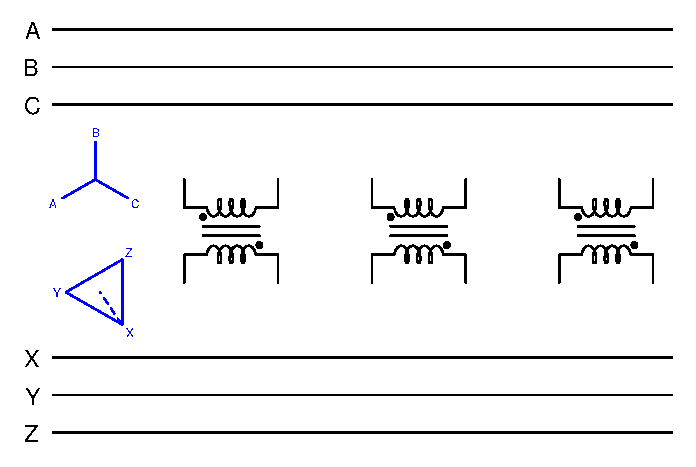
\includegraphics[width=15.5cm]{i00848x01.eps}$$

Oppgi også fasefølgen (faserotasjon) for begge trefaseskinner, og identifiser om nedre skinne {\it leder}, {\it henger etter}, eller er {\it i fase} med øvre skinne.

\underbar{file i00848}
%(END_QUESTION)





%(BEGIN_ANSWER)

Dette er ikke den eneste løsningen, men den fungerer. Merk prikkene og tallene i fasordiagrammene for å holde oversikt over hvilke transformatorer og polariteter som brukes:

$$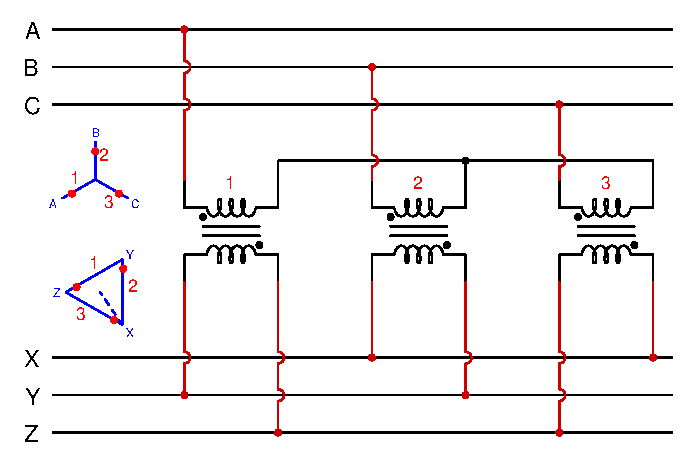
\includegraphics[width=15.5cm]{i00848x02.eps}$$

Fasefølgen på øvre skinne er ABC.

\vskip 10pt

Fasefølgen på nedre skinne er ZYX.

\vskip 10pt

Faseforskyvningen mellom skinnene (sammenlign $V_A$ med $V_X$) er 90$^{o}$, der nedre skinne {\it leder} øvre skinne: $V_A = \angle -150^o$ og $V_X = \angle -60^o$

%(END_ANSWER)





%(BEGIN_NOTES)


%INDEX% Electronics review, 3-phase transformer bank phase shift calculations

%(END_NOTES)
